\chapter{Overview of Method and Tools Used}\label{ch:method}

\section{Method overview}
The aim of this thesis is to provide sound designers with an easy-to-use tool which enriches video games with procedural and physics-based audio instead of having to use prerecorded sounds. The tool enables to control contact sounds (impact, rolling and scratching) produced by vibrating objects through high level parameters that characterize the objects (size, material and surface roughness). The challenge is to offer realistic real-time and event-based sounds in a game engine without high gls{CPU} usage.

\Todo{replace figure  with a better one}
\begin{figure}[H]
  \centering
    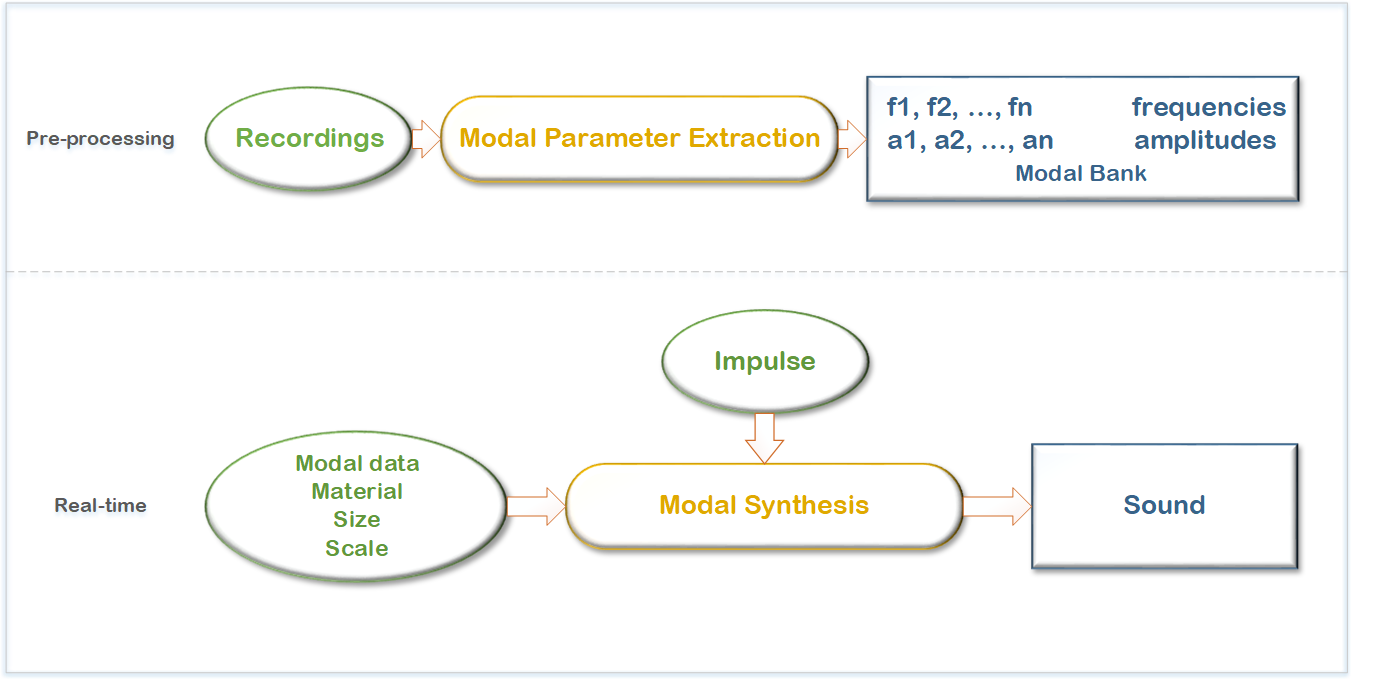
\includegraphics[width=\textwidth]{overview.png}
      \caption{Tool overview.}
      \label{fig:synth_proc}
\end{figure}

To create this tool, the procedure described in figure \ref{fig:synth_proc} was followed. To extract the modal parameters of vibrating objects the ``Example-guided'' method described in \ref{sec:exampleguided} was used due to its better integration within the audio pipeline as opposed to the rest of techniques presented in \ref{sec:modal_extraction}. The first step was to find several everyday objects that were made of different materials (plastic, wood, ceramic, glass and metal). This is because a priority in this thesis is the synthesis of sounds based on material properties. To obtain sound variations along the object's surface (see second method in \ref{sec:sound_variation}) the chosen objects were divided into areas that produced similar sounds when struck (e.g. bottle neck, rim of glass, etc). Between two and six sounds were recorded depending on the object. An example is presented in the following section for illustration \ref{sec:recordings}.

In the pre-processing stage, the recordings were then used to extract the data needed for the sound synthesis with the ChucK programming language. Some involved \gls{DSP} algorithms that employ the \gls{FFT} are used to capture the modal frequencies and gains specific of the object and which are present in the supplied audio clips. This process is explained in more depth in section \ref{sec:chuck}. 

As far as the modal synthesis of impact sounds is concerned, the two methods shown in \ref{sec:modal_synth} have been implemented into Pure Data patches \ref{sec:impact_synth} to evaluate differences between the output sounds. Scratching and rolling sounds (see \ref{sec:scratching_synth} and \ref{sec:rolling_synth} respectively) also make use of the filter-based method.

3D models of the recorded real world objects were generated in Maya \cite{bib:maya}. The models were then combined with their corresponding modal data and synthesis patches inside Unity\textsuperscript{\textregistered} software. Heavy was used to generate audio plugins from the Pd patches for better integration in the game engine and interactivity with the synthesizer. 

At runtime, rigid-body physics events have been used to drive the synthesizer. Depending on the interaction (impact, rolling or scratching) the model is excited differently and produces the corresponding sound which is tightly coupled with the graphics. The final stage of the audio chain is the spatialization which is done with Unity's Audio Spatializer SDK \cite{bib:unity_doc}.

\section{Sound discretization scheme}\label{sec:discretization}

The first step for the creation of this tool is to obtain the necessary data for the audio synthesis through the use of the ``Example-guided'' method as mentioned in \ref{sec:exampleguided}. This method was applied instead of the \gls{FEM}, as in \cite{director2001synthesizing} and \cite{o2002synthesizing}, or the spring-mass systems method as in \cite{raghuvanshi2006interactive} because of its simplicity within an audio pipeline in a video game production. More specifically, the usage of recordings is an easier option for the targeted users (sound designers and game developers) than one that implies complex computations of vibrating structures. Additionally, Unity\textsuperscript{\textregistered} seems to present some limitations for techniques that present sound variation depending on vertex collisions such as the \gls{FEM} and spring-mass systems. The game engine is not able to provide the exact vertex that has collided. 

To produce sound variations along the surface of an object, a method is to have only one amplitude matrix (corresponding to only one point of the object) and randomize the values every time a collision occurs. During the development of this thesis we tried this method, but we abandoned it rather quickly due to undesirable sounding results. In other words, two impact sounds, being produced by two very close locations on the object, were exceptionally different. Thus, recordings of the sound produced by everyday objects when hit in several locations were performed instead. The strategy used is explained in detail in section \ref{sec:recordings}.

The objects recorded were chosen due to their simple shape and symmetry plus the fact that they are easy to find in most kitchens. A heuristic approach that assumes that nearby points produce almost the same sound was adopted. This lead to the division of the object into ``sound areas'' instead of calculating different modal matrices for each vertex of the model as in the \gls{FEM}. Unofficial audio tests proved that this complexity-accuracy trade-off was acceptable to map the different sound variations along the struck object's surface. Depending on the range of substantially different sounds produced by the object, more or less areas were chosen. A sample object and its division in areas is shown in figure \ref{fig:pot_sep}. 

\begin{figure}[H]
  \centering
    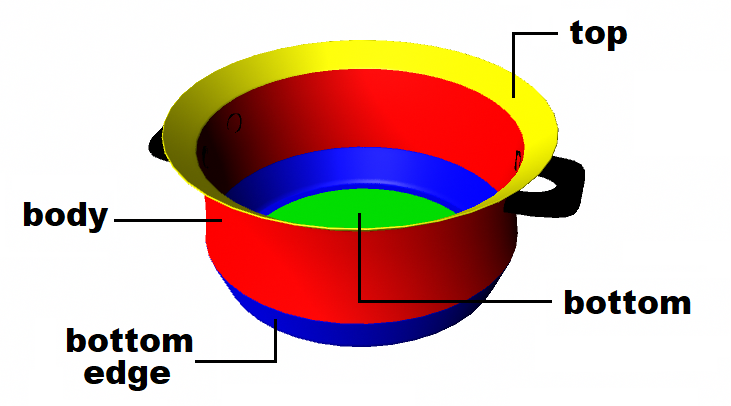
\includegraphics[width=0.6\textwidth]{potseparated.png}
      \caption{Division of an object into areas with similar sound.}
      \label{fig:pot_sep}
\end{figure} 

\section{3D models}

For coherence purposes the objects recorded were modeled so that the synthetic sounds match with the 3D model, the same way the recordings match with the real world objects. Hence, the dimensions and weight of the eleven objects were measured to model the objects. In table \ref{tab:dim_weig} the maximum dimensions and the weight of the objects are displayed. Maya Autodesk software was used to create the 3D models of the objects. They were exported as FBX\textsuperscript\textregistered\ files \cite{bib:fbx} which is a format recognizable by Unity\textsuperscript{\textregistered}.

\begin{table}[H]
	\centering
    \begin{tabular}{ l c r c}
    \toprule
    \textbf{Name} & \textbf{Dimensions(cm)} & \textbf{Weight(g)} & \textbf{Picture} \\
    \toprule 
    Cooking pot & $21.5L\times 21.5W\times 10.8H$ & 680 & 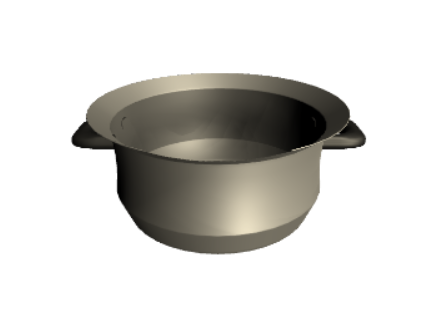
\includegraphics[scale=0.1]{3DmodelsPics/cp.PNG} \\ 
    Cup & $7.5L\times 7.5W\times 6H$ & 125 & 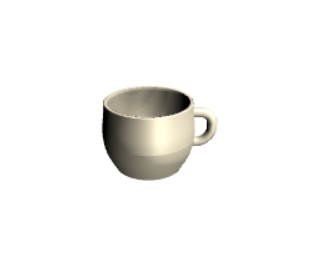
\includegraphics[scale=0.1]{3DmodelsPics/cup.PNG} \\ 
    Cutting board & $41.5L\times 26.5W\times 4.5H$ & 2200 & 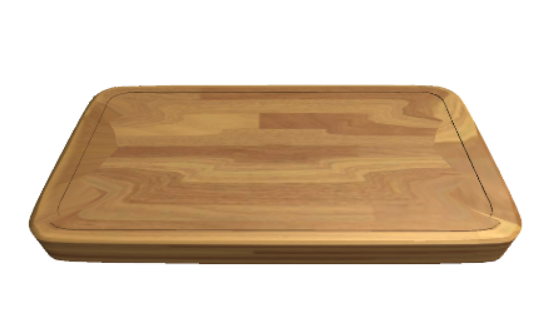
\includegraphics[scale=0.1]{3DmodelsPics/cb.PNG} \\ 
    Jug & $14L\times 10W\times 21.5H$ & 150 & 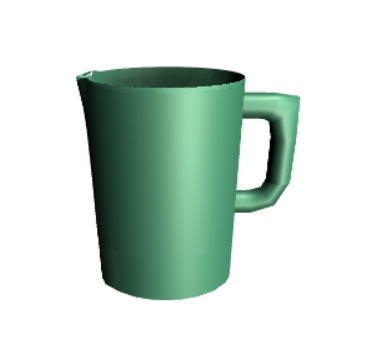
\includegraphics[scale=0.1]{3DmodelsPics/jug.PNG} \\ 
    Mortar & $11L\times 11W\times 19H$ & 850 & 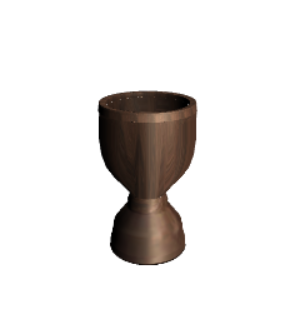
\includegraphics[scale=0.1]{3DmodelsPics/mortar.PNG} \\
    Bowl & $20L\times 20W\times 10.5H$ & 100 & 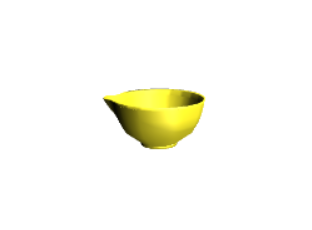
\includegraphics[scale=0.1]{3DmodelsPics/bowl.PNG} \\
    Plate & $25.5L\times 25.5W\times 2.5H$ & 700 & 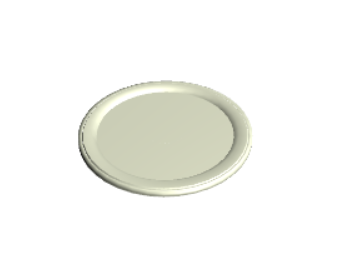
\includegraphics[scale=0.1]{3DmodelsPics/plate.PNG} \\
    Rolling pin & $43L\times 7W\times 7H$ & 700 & 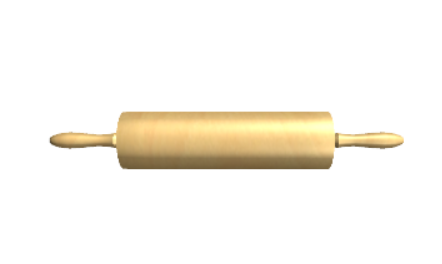
\includegraphics[scale=0.1]{3DmodelsPics/rp.PNG} \\
    Wine bottle & $7L\times 7W\times 29H$ & 400 & 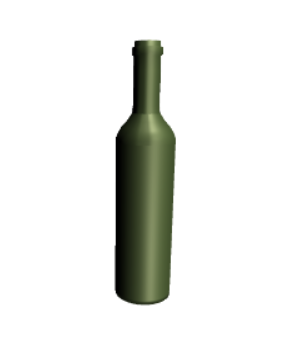
\includegraphics[scale=0.1]{3DmodelsPics/bottle.PNG} \\
    Wine glass & $8L\times 8W\times 18H$ & 120 & 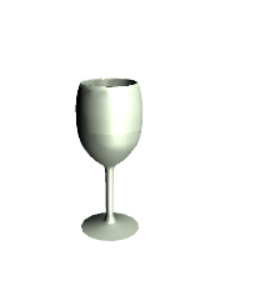
\includegraphics[scale=0.1]{3DmodelsPics/glass.PNG} \\
    Wok & $35L\times 35W\times 9.5H$ & 1225 & 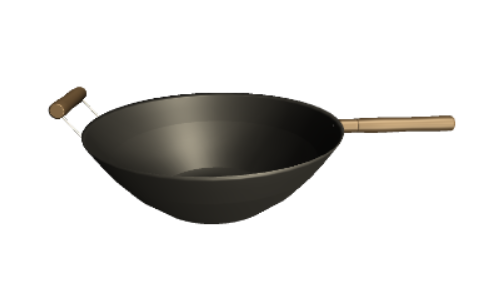
\includegraphics[scale=0.1]{3DmodelsPics/wok.PNG} \\
    \bottomrule
    \end{tabular}
    \caption{Maximun dimensions and weight of the eleven objects.}
    \label{tab:dim_weig}
\end{table}

%     \begin{minipage}{.45\textwidth}
%      \begin{itemize}
%        \item Cooking Pot
%		\item Cup
%		\item Cutting Board
%		\item Jug
%		\item Mortar
%		\item Bowl
%		\item Plate
%		\item Rolling Pin
%		\item Wine Bottle
%		\item Wine Glass
%		\item Wok
%     \end{itemize}
%  \end{minipage}
%    \begin{minipage}{.45\textwidth}
%    	\hspace{-3cm}
%    		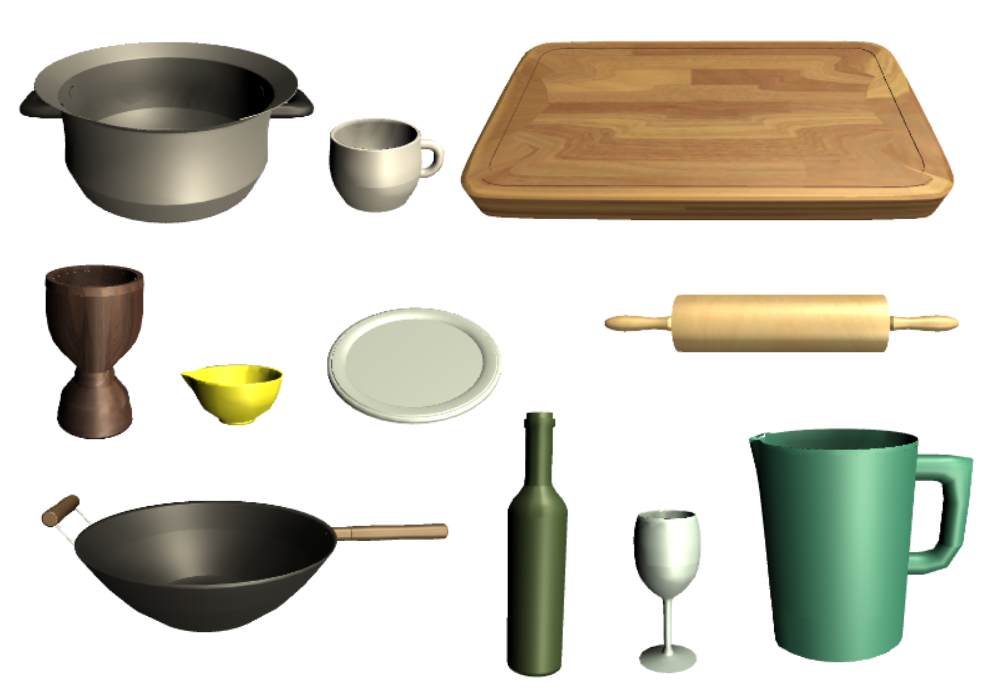
\includegraphics[scale=0.4]{3DmodelsPics/3dmodels.png}
%     		 \label{fig:3d_all}
%    \end{minipage}

\section{Modal data extraction}\label{sec:chuck}

The ChucK language is a music programming language, made for ``real-time sound synthesis and music creation'' as mentioned in their website \cite{bib:chuck}. It's biggest advantage is the way it manipulates time. More specifically, the user specifies how long a sound will last, independently of other sounds that may be playing at the same time.

 %Other options to analyze and synthesize sounds are the Python programming language or the Csound API but they both demand involved computations. %
ChucK was chosen for this stage of the work, because of its built-in functions to manipulate sound, like the \textit{Fast Fourier Transform (FFT)} and windowing of input audio signals \cite{bib:chuck_doc}. The algorithm used in this part of the thesis is made by Perry Cook for the course \textit{Physics-Based Sound Synthesis for Games and Interactive Systems} held by Perry Cook and Julius O. Smith at Kadenze Academy \cite{bib:physicsbasedcourse}. The ChucK language was used to identify and extract the frequency modes and gains of the recorded audio files. The output provided by this code therefore delivers exactly the parameters needed for modal synthesis. The aforementioned course is the main reason behind the choice of this programming language.

When analyzing the recordings one can identify that each object has a very high number of resonant modes. Although, most of them are inaudible and do not contribute significantly to the sound model. It is, therefore, desirable to preserve CPU cycles by reducing the number of calculated modes. Based on the recommendations of the author, Perry Cook, ten modes were chosen as the sufficient amount for the analysis/synthesis. Afterwards, the algorithm having taken a recording as input, computes an histogram and identifies the modes. The frequencies where peaks occur are the modal frequency candidates. Depending on the numbers of modes chosen, the algorithm outputs the most relevant ones. Finally, the algorithm calculates after a normalization process the corresponding amplitude of each mode.


\Todo{should we explain why we used FFT?} 
 
\section{Modal synthesis patches}

Pure Data (Pd) is another music programming language. It is open source and the main difference with the ChucK language is that \gls{Pd} is a visual or ``patcher'' programming language, using objects instead of code, linked together to form a sequence \cite{bib:pd}. This software was chosen as our synthesis engine mainly because of the ability to compile the patches into C\# code, as explained below in section \ref{sec:heavy}. Another important reason for choosing it is the possibility of real-time parameter manipulation and easy testing during the implementation period.

All synthesized sounds (impact, rolling and scratching) are synthesized under one main pd patch. However, two different patches have been developed, one for each of the two examined methods. Since the audio synthesis patch takes the modal data as input, every object can use the same patch. The synthesis patches will be described in detail in section \ref{sec:synthesis_implem}.

%For optimization reasons, we lowered the number of modes down to 10 instead of 20 that we initially had, since the extra 10 did not add any useful information to the output sound. In addition, we clipped the range of frequencies to the human audible range of 20Hz to 20KHz. 

\Todo{develop more?}

\section{Audio plugins}\label{sec:heavy}

Heavy is a compiler that generates audio plugins from \gls{Pd} patches in interactive sound and music applications \cite{bib:heavy}. In this thesis it is used it to compile \gls{Pd} patches into Unity\textsuperscript{\textregistered} audio plugins. Heavy's interface is a website where users upload patches and then are able to download the corresponding plugins and put them into their applications. The plugins used consist of DLL files and a C\# (Unity\textsuperscript{\textregistered} code) script that allows communication of the plugins with the rest of the scripts and also enables the sound card to play audio.

Through the generated C\# script, we are able to send float values to the audio plugins - which are the compiled \gls{Pd} patches - as inputs to generate the appropriate sound. Those floats are the frequencies and their corresponding amplitudes, the quality factor (\gls{Q}) of the band-pass filters, the impact force of the collision, the roughness of the object, the multiplier of the size of the object, the velocity of the object and the rolling and scratching duration times. A difficulty encountered while using this compiler was the inability of sending a whole array or list of floats. Thus, we had to send every frequency and every amplitude individually, creating a float parameter for each.
 
\subsection{Why not OSC?}
The most popular way to communicate between Unity\textsuperscript{\textregistered} and \gls{Pd} is the Open Sound Control (OSC) protocol. The reason why we did not use it is because it requires establishing a connection between two software programs and send data between them. On the other hand, Heavy makes everything work inside Unity\textsuperscript{\textregistered} and it is as simple as passing floats between scripts. 

\section{Game engine}
Unity\textsuperscript{\textregistered} is a game engine software. This is where all previous work is combined together and the final product is delivered. For the purpose of this thesis, several demonstration scenes are made inside Unity\textsuperscript{\textregistered} where objects are struck in several points and suffer different interactions while producing different sounds. 

Unity\textsuperscript{\textregistered} was chosen due to its ease of use, cross-platform publishing compatibility, intuitive collision events and because the authors have experience developing games with this game engine. Additionally, Unity\textsuperscript{\textregistered} is the only game engine that is supported by Heavy.

The first part of the Unity\textsuperscript{\textregistered} implementation is the assignment of modal data to every different area of the object. This is done in linear time ($O(n)$ for $n$ modes). The whole procedure of assigning the appropriate data includes the identification of the area of the object that collided, filling the arrays with the corresponding data and set the parameters of the plugins. Afterwards, the type of collision is identified and a number of other parameters are calculated and sent to the plugins, like the impact force and the duration of the collision.

Audio in Unity\textsuperscript{\textregistered} is enabled using the \textit{OnAudioFilterRead()} function. This function is running in the audio thread, which is a different one from the main thread. Its job is to send the audio buffer to the sound card and is called every $\sim 20$ms, so it does not require a function call from the programmer \cite{bib:unity_doc}.

\section{Sound spatialization}

In this paper the sound spatialization is considered a separate process with respect to the sound synthesis. This approach was considered due to the Audio Spatializer SDK provided by Unity\textsuperscript{\textregistered} which delivers the desired effect.

The Audio Spatializer SDK is a plugin that replaces the standard panner in Unity\textsuperscript{\textregistered} by a more advanced one \cite{bib:unity_doc}. It makes use of \gls{HRTF} filtering which is based on the KEMAR data set \cite{kemar}, an extensive library of \GLS{HRTF} measurements on a dummy head microphone by Bill Gardner and Keith Gardner at MIT Media Lab. The Audio Spatializer SDK changes how the audio is transmitted so that it seems like the listener is in a 3D environment. Depending on the position of the listener in the virtual scene and the audio source, the spatializer adjusts the left and right channel gains to simulate a virtual sound field.

\section{Microsoft Hololens Emulator}
\Todo{keep it or not?}

